\chapter{Separating Mixtures}\label{ch:g3:separating-mixtures}

After a storm, the puddles in the road are brown: rain water mixed with
soil, sand and bits of leaves. Yet the water that comes out of a kitchen
tap is clear, and it too was rain once, before it ran into a river. How
can muddy water be made clean again? Things that have been mixed can be
taken apart. This chapter shows how, one method at a time.

\begin{recall}
To \omterm{def:g2:mixing-and-dissolving:mix}{mix} is to put different things together. A solid such as sugar or
salt \omterm{def:g2:mixing-and-dissolving:dissolve}{dissolves} in water: it disappears from sight, and the clear liquid
is a solution. A dissolved solid is still there: when the water dries
away, the solid is left behind. Sand and soil do not \omterm{def:g2:mixing-and-dissolving:dissolve}{dissolve}
(\cref{ch:g2:mixing-and-dissolving}).
\end{recall}

\section{Sorting by hand and sieving}

When the pieces of a \omterm{def:g2:mixing-and-dissolving:mix}{mix} are big enough to see and to pick up, the
simplest way to separate them is by hand: raisins can be picked out of
muesli one by one. When there are too many pieces, a sieve does the
sorting for us.

\begin{definition}[Sieving]\label{def:g3:separating-mixtures:sieve}
\emph{Sieving}\index{sieving} is separating the pieces of a \omterm{def:g2:mixing-and-dissolving:mix}{mix} by
their size, with a sieve: a net or a plate full of holes. The small
pieces fall through the holes; the big pieces stay in the sieve.
\end{definition}

\begin{example}[Gravel and sand]\label{ex:g3:separating-mixtures:gravel}
A builder shakes a \omterm{def:g2:mixing-and-dissolving:mix}{mix} of gravel and sand over a sieve. The fine sand
falls through into a heap below; the gravel stays on the mesh.
\end{example}

\begin{omfigure}
\begin{tikzpicture}[font=\small]
  % the sieve: a mesh bowl
  \fill[pattern=crosshatch, pattern color=black!45] (-1.6,2.6) arc[start angle=180,
    end angle=360, x radius=1.6, y radius=0.7] -- cycle;
  \draw[black!70, line width=0.8pt] (-1.6,2.6) arc[start angle=180, end angle=360,
    x radius=1.6, y radius=0.7];
  \draw[black!70, line width=0.8pt] (-1.75,2.6) -- (1.75,2.6);
  \draw[black!70, line width=1.4pt] (1.75,2.6) -- (3.0,2.85);
  % gravel kept in the sieve
  \foreach \x/\y/\r in {-0.9/2.25/0.17,-0.45/2.12/0.2,0.05/2.08/0.18,0.5/2.13/0.21,
                        0.95/2.28/0.16,-0.2/2.42/0.15,0.3/2.43/0.17}
    \fill[black!45, draw=black!65] (\x,\y) circle (\r);
  % sand falling
  \foreach \x/\y in {-0.4/1.6,0.1/1.4,0.4/1.7,-0.15/1.15,0.25/1.0,-0.5/0.95,0.0/0.75}
    \fill[orange!60!brown] (\x,\y) circle (0.05);
  % the heap of sand in a bowl
  \fill[orange!45!brown!70] (-1.0,0.12) .. controls (-0.5,0.55) and (0.5,0.55)
    .. (1.0,0.12) -- cycle;
  \draw[black!70, line width=0.8pt] (-1.5,0.5) .. controls (-1.3,0) and (1.3,0)
    .. (1.5,0.5);
  \node[anchor=west] at (2.0,2.2) {the gravel stays in the sieve};
  \node[anchor=west] at (2.0,1.25) {the sand falls through the holes};
  \node[anchor=west] at (2.0,0.3) {a heap of sand};
\end{tikzpicture}

{\small \omterm{def:g3:separating-mixtures:sieve}{Sieving} a \omterm{def:g2:mixing-and-dissolving:mix}{mix} of gravel and sand: the pieces are sorted by their
size.}
\end{omfigure}

\begin{omfigure}
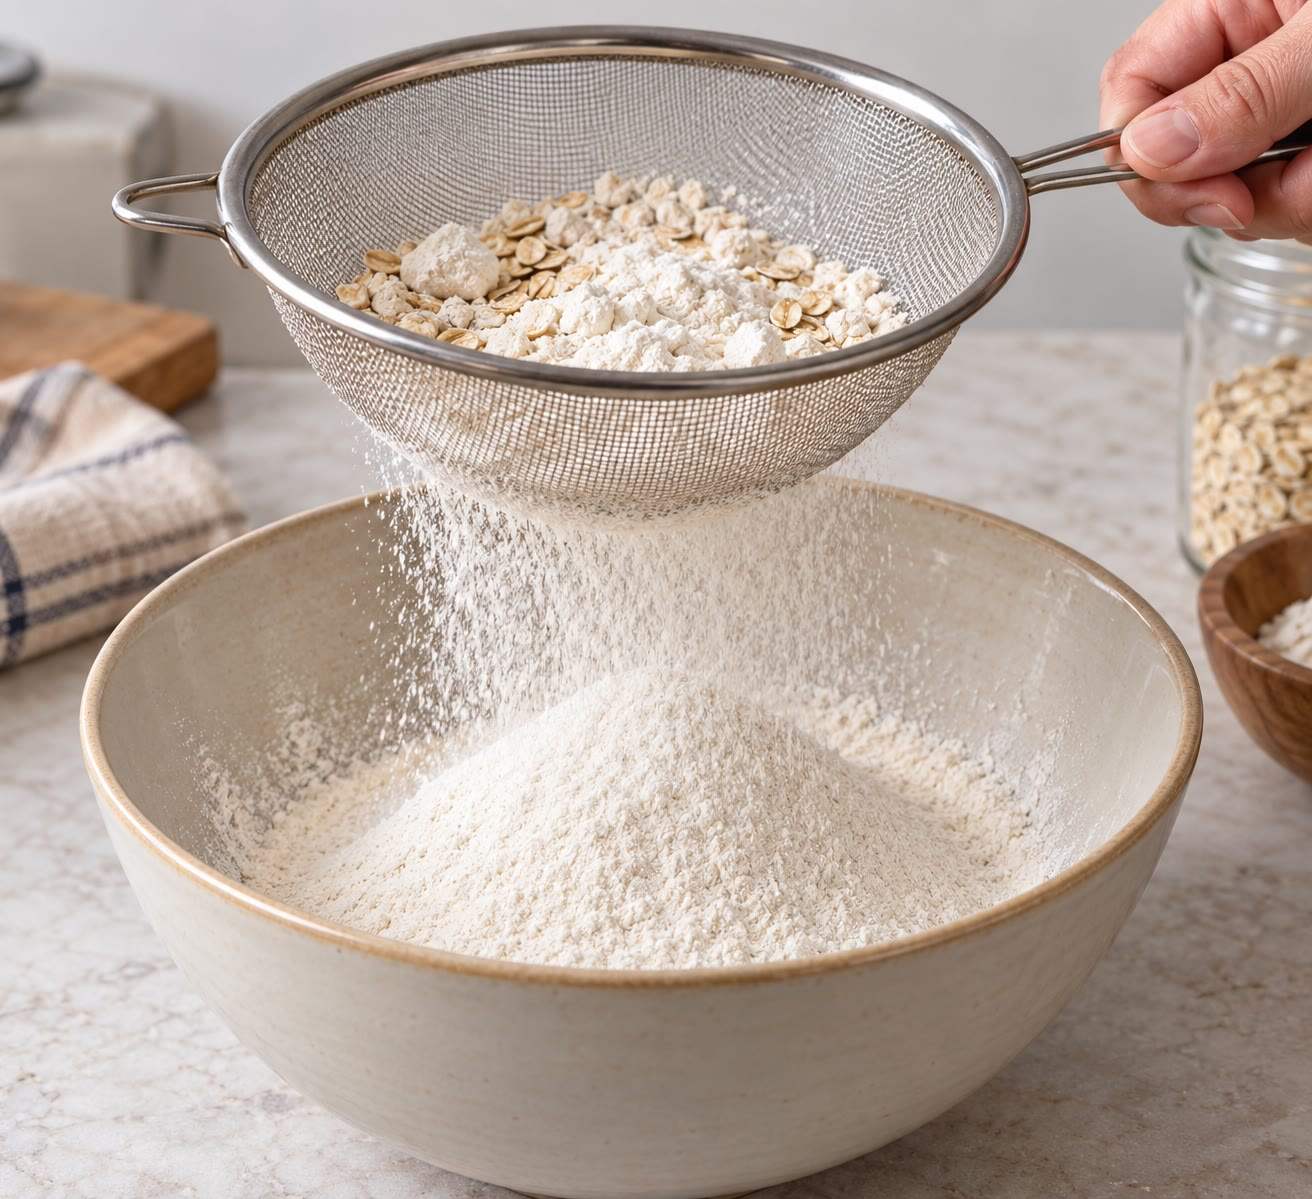
\includegraphics[width=0.55\linewidth]{images/book1/ai/g3-kitchen-sieve.jpg}

{\small A kitchen sieve: the fine flour goes through, the lumps stay
behind.}
\end{omfigure}

\section{Letting settle and decanting}

\begin{definition}[Settling and decanting]\label{def:g3:separating-mixtures:decant}
A \omterm{def:g2:mixing-and-dissolving:mix}{mix} of water and of a solid that does not \omterm{def:g2:mixing-and-dissolving:dissolve}{dissolve} can be left to
rest: the solid sinks slowly to the bottom. This is called
\emph{settling}\index{settling}. Once it has settled, the clear water
above can be poured gently into another container, leaving the solid
behind: this is \emph{decanting}\index{decanting}.
\end{definition}

\begin{omfigure}
\begin{tikzpicture}[font=\small]
  % 1: stirred, cloudy
  \pic at (0,0) {beaker={0.7}{brown!28}};
  \foreach \x/\y in {-0.5/0.3,-0.2/0.6,0.3/0.4,0.5/0.9,-0.4/1.0,0.1/1.2,0.4/0.15,
                     -0.1/0.25,0.2/0.8,-0.55/0.7}
    \fill[brown!60] (\x,\y) circle (0.03);
  \node[anchor=north, align=center] at (0,-0.15) {stirred:\\ cloudy};
  \draw[->, thick, omProp] (1.1,1.0) -- (2.4,1.0);
  % 2: settled
  \pic at (3.5,0) {beaker={0.7}{omWater!80}};
  \fill[brown!60] (2.7,0) rectangle (4.3,0.25);
  \draw[omGlass, line width=0.7pt] (2.7,0.25) -- (2.7,0) -- (4.3,0) -- (4.3,0.25);
  \node[anchor=north, align=center] at (3.5,-0.15) {left to rest:\\ the soil has settled};
  \draw[->, thick, omProp] (4.6,1.0) -- (5.9,1.0);
  % 3: decanted
  \pic at (7.0,0) {beaker={0.1}{omWater!80}};
  \fill[brown!60] (6.2,0) rectangle (7.8,0.25);
  \draw[omGlass, line width=0.7pt] (6.2,0.25) -- (6.2,0) -- (7.8,0) -- (7.8,0.25);
  \pic at (9.2,0) {beaker={0.58}{omWater!80}};
  \node[anchor=north, align=center] at (8.1,-0.15) {poured off: clear water\\ on the right, soil left behind};
\end{tikzpicture}

{\small \omterm{def:g3:separating-mixtures:decant}{Settling}, then \omterm{def:g3:separating-mixtures:decant}{decanting} a \omterm{def:g2:mixing-and-dissolving:mix}{mix} of soil and water.}
\end{omfigure}

\begin{remark}[Settling takes time]\label{rem:g3:separating-mixtures:time}
Big, heavy grains settle in a few minutes; very fine clay can take a day
or more, and the water stays a little cloudy meanwhile. \omterm{def:g3:separating-mixtures:decant}{Decanting} never
removes every grain: a little cloudiness is poured off with the water.
\end{remark}

\section{Filtering}

\begin{definition}[Filtering and filtrate]\label{def:g3:separating-mixtures:filter}
\emph{Filtering}\index{filtering} is pouring a \omterm{def:g2:mixing-and-dissolving:mix}{mix} through a filter: a
sheet of paper, a cloth or a layer of sand with holes too small to let
the solid pieces through. The solid stays on the filter; the clear
liquid that passes through is called the
\emph{filtrate}\index{filtrate}.
\end{definition}

\begin{omfigure}
\begin{tikzpicture}[font=\small, scale=1.4]
  \pic[transform shape] at (0,0) {beaker={0.35}{omWater!80}};
  \pic[transform shape] at (0,1.4) {funnel={brown!55}};
  % muddy water waiting in the paper cone, above the soil
  \fill[brown!25] (-0.411,2.45) -- (0.411,2.45) -- (0.722,2.8) -- (-0.722,2.8) -- cycle;
  % drops of filtrate
  \foreach \y in {1.15,0.95} \fill[omDef!50] (0,\y) circle (0.04);
  \draw[<-, omProp, thick] (0.75,2.6) -- (2.0,2.9) node[right, text=black]
    {filter paper in a funnel};
  \draw[<-, omProp, thick] (0.25,2.15) -- (2.0,2.2) node[right, text=black]
    {the soil stays on the paper};
  \draw[<-, omProp, thick] (0.85,0.4) -- (2.0,0.6) node[right, text=black]
    {the filtrate: clear water};
\end{tikzpicture}

{\small \omterm{def:g3:separating-mixtures:filter}{Filtering} muddy water through a paper filter.}
\end{omfigure}

\begin{inthelab}[Filtering muddy water]
The teacher folds a round sheet of filter paper into a cone and sets it
in a glass funnel above a beaker. Muddy water is poured into the cone, a
little at a time, never above the edge of the paper. Clear water drips
into the beaker; the soil makes a brown layer on the paper. When the
\omterm{def:g3:separating-mixtures:filter}{filtrate} is cloudy, the paper is torn or the water went over its edge.
\end{inthelab}

\begin{proposition}[A filter does not stop what is dissolved]\label{prop:g3:separating-mixtures:dissolved}
A filter holds back the solid pieces that are not dissolved. It does not
hold back what is dissolved: salty water poured through a filter comes
out just as salty, and sweet tea just as sweet.
\end{proposition}

\begin{omfigure}
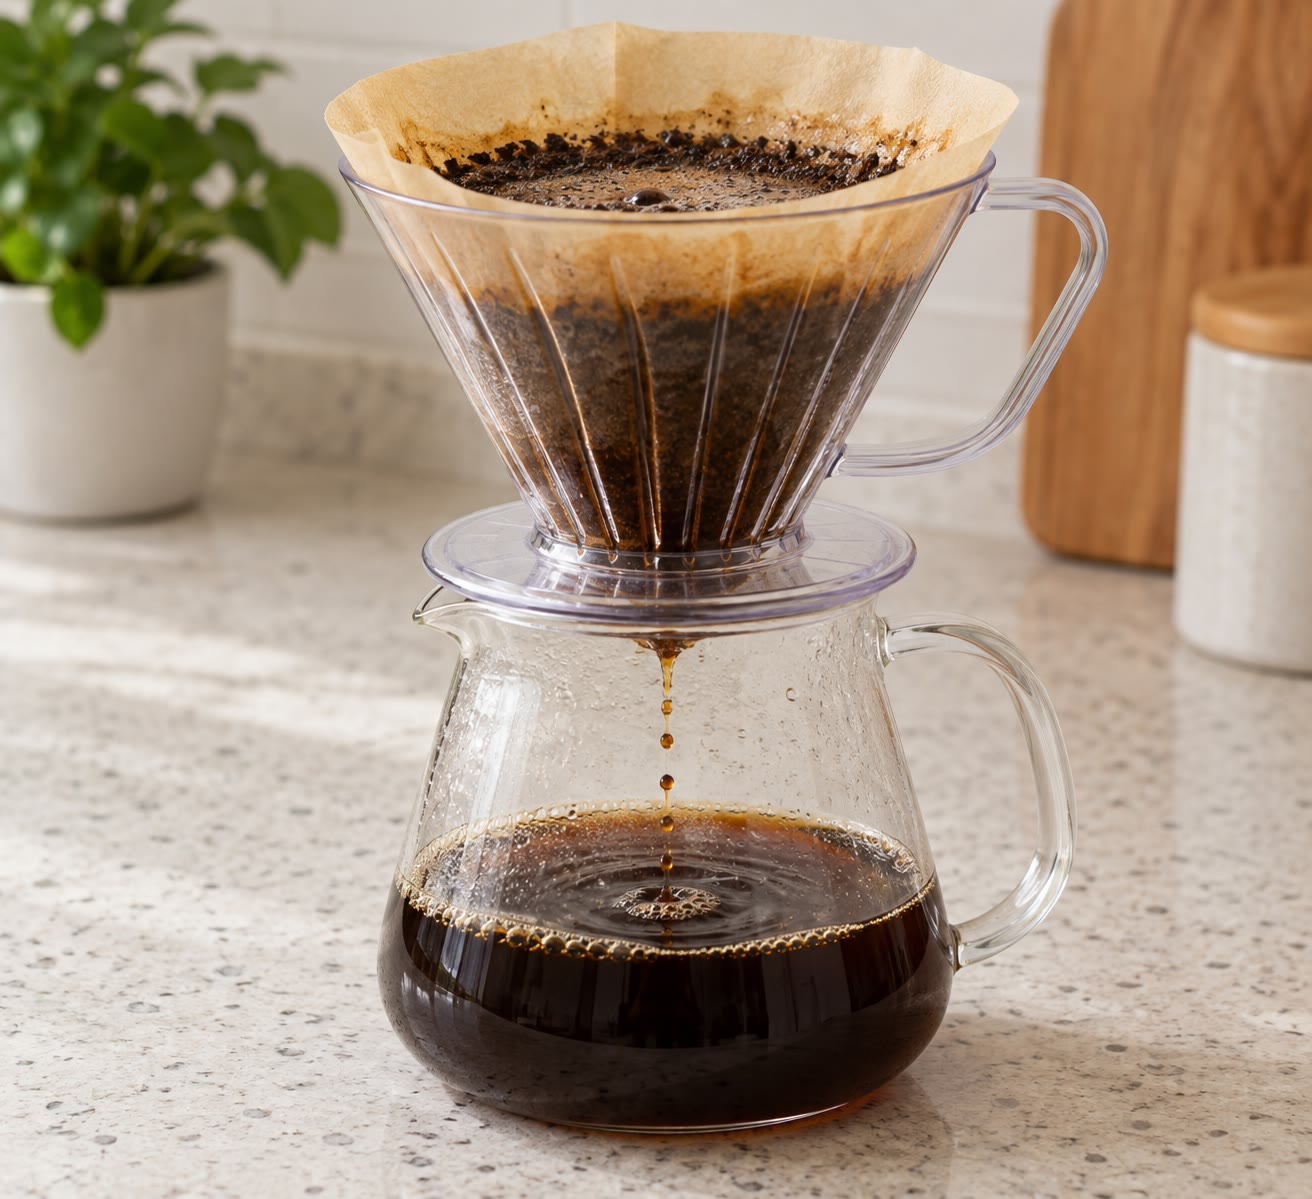
\includegraphics[width=0.5\linewidth]{images/book1/ai/g3-coffee-filter.jpg}

{\small Making coffee is \omterm{def:g3:separating-mixtures:filter}{filtering}: the grounds stay in the paper, the
coffee is the \omterm{def:g3:separating-mixtures:filter}{filtrate}.}
\end{omfigure}

\section{Evaporating the water away}

\begin{definition}[Evaporating]\label{def:g3:separating-mixtures:evaporate}
To get back a solid that is dissolved in water, the water is left to dry
away, in the sun or on a gentle heat: this is
\emph{evaporating}\index{evaporating}. The water goes into the air; the
solid stays in the dish.
\end{definition}

\begin{example}[Salt from salty water]\label{ex:g3:separating-mixtures:salt}
A little salty water is poured into a shallow dish and left on a sunny
window sill. Days later there is no water left, only a white crust of
salt: the salt that was dissolved.
\end{example}

\begin{omfigure}
\begin{tikzpicture}[font=\small, scale=1.4]
  \pic[transform shape] at (0,0) {hotplate};
  \pic[transform shape] at (0,0) {evapdish={omWater!80}};
  \node[anchor=north, align=center] at (0,-0.6) {salty water,\\ gently heated};
  \draw[->, thick, omProp] (1.5,0.3) -- (3.0,0.3) node[midway, above, text=black]
    {later};
  \pic[transform shape] at (4.5,0) {hotplate};
  \pic[transform shape] at (4.5,0) {evapdish={white!85!black}};
  \foreach \x in {-0.45,-0.25,-0.05,0.15,0.35}
    \fill[white, draw=black!45, line width=0.2pt] (4.5+\x,0.12) rectangle ++(0.09,0.06);
  \node[anchor=north, align=center] at (4.5,-0.6) {no water left:\\ salt crystals};
  \foreach \x in {-0.3,0,0.3} \draw[->, black!45, decorate,
    decoration={snake, amplitude=0.6pt, segment length=4pt}] (\x,0.7) -- (\x,1.4);
  \node[anchor=south] at (0,1.4) {water goes into the air};
\end{tikzpicture}

{\small \omterm{def:g3:separating-mixtures:evaporate}{Evaporating}, in the laboratory: the dish is warmed gently on a
hotplate by the teacher. The salt stays in the dish.}
\end{omfigure}

\section{Which method for which mixture?}

\begin{method}[Choosing a separation]\label{met:g3:separating-mixtures:choose}
To take a \omterm{def:g2:mixing-and-dissolving:mix}{mix} apart, ask:
\begin{enumerate}
  \item Are the pieces big and of different sizes? Sort by hand, or
        sieve.
  \item Is there a solid that does not \omterm{def:g2:mixing-and-dissolving:dissolve}{dissolve}, in a liquid? Let it
        settle and decant, or filter for clearer water.
  \item Is there a solid dissolved in the liquid? Evaporate the liquid:
        the solid stays.
\end{enumerate}
Several steps are often needed, one after the other.
\end{method}

\begin{example}[Sand, salt and water]\label{ex:g3:separating-mixtures:three}
A jar holds water with sand and salt in it. The salt has dissolved; the
sand has not.
\begin{enumerate}
  \item Filter: the sand stays on the paper.
  \item The \omterm{def:g3:separating-mixtures:filter}{filtrate} is clear, but it is salty water. Evaporate it: the
        salt stays in the dish.
\end{enumerate}
Two methods, one after the other, give back the sand and the salt.
\end{example}

\begin{example}[Clean water from a river]\label{ex:g3:separating-mixtures:plant}
A water-treatment plant makes river water fit to drink in several steps:
\begin{enumerate}
  \item the river water passes through screens, big grids that stop
        branches, leaves and plastic: a kind of \omterm{def:g3:separating-mixtures:sieve}{sieving};
  \item it rests in large tanks where mud settles to the bottom;
  \item it is filtered through thick beds of sand that hold back the
        finest grains;
  \item a very small amount of a product that kills germs is added, so
        that the water stays safe in the pipes.
\end{enumerate}
\end{example}

\begin{omfigure}
\begin{tikzpicture}[font=\small, node distance=0.45cm,
    box/.style={draw=omDef, fill=omDef!6, rounded corners=2pt, align=center,
      minimum height=1.15cm, text width=2.0cm}]
  \node[box] (r) {river\\ water};
  \node[box, right=of r] (s) {screens\\ (sieving)};
  \node[box, right=of s] (t) {settling\\ tanks};
  \node[box, right=of t] (f) {sand\\ filters};
  \node[box, right=of f] (g) {germs\\ killed};
  \foreach \a/\b in {r/s,s/t,t/f,f/g} \draw[->, thick, omProp] (\a) -- (\b);
  \node[below=0.15cm of s, font=\footnotesize, align=center] {branches,\\ plastic};
  \node[below=0.15cm of t, font=\footnotesize, align=center] {mud};
  \node[below=0.15cm of f, font=\footnotesize, align=center] {fine grains};
  \draw[->, thick, omProp] (g.south) -- ++(0,-0.8) node[below] {to the taps};
\end{tikzpicture}

{\small The steps of a water-treatment plant. Under each step: what it
removes.}
\end{omfigure}

\begin{omfigure}
\begin{minipage}[t]{0.48\linewidth}\centering
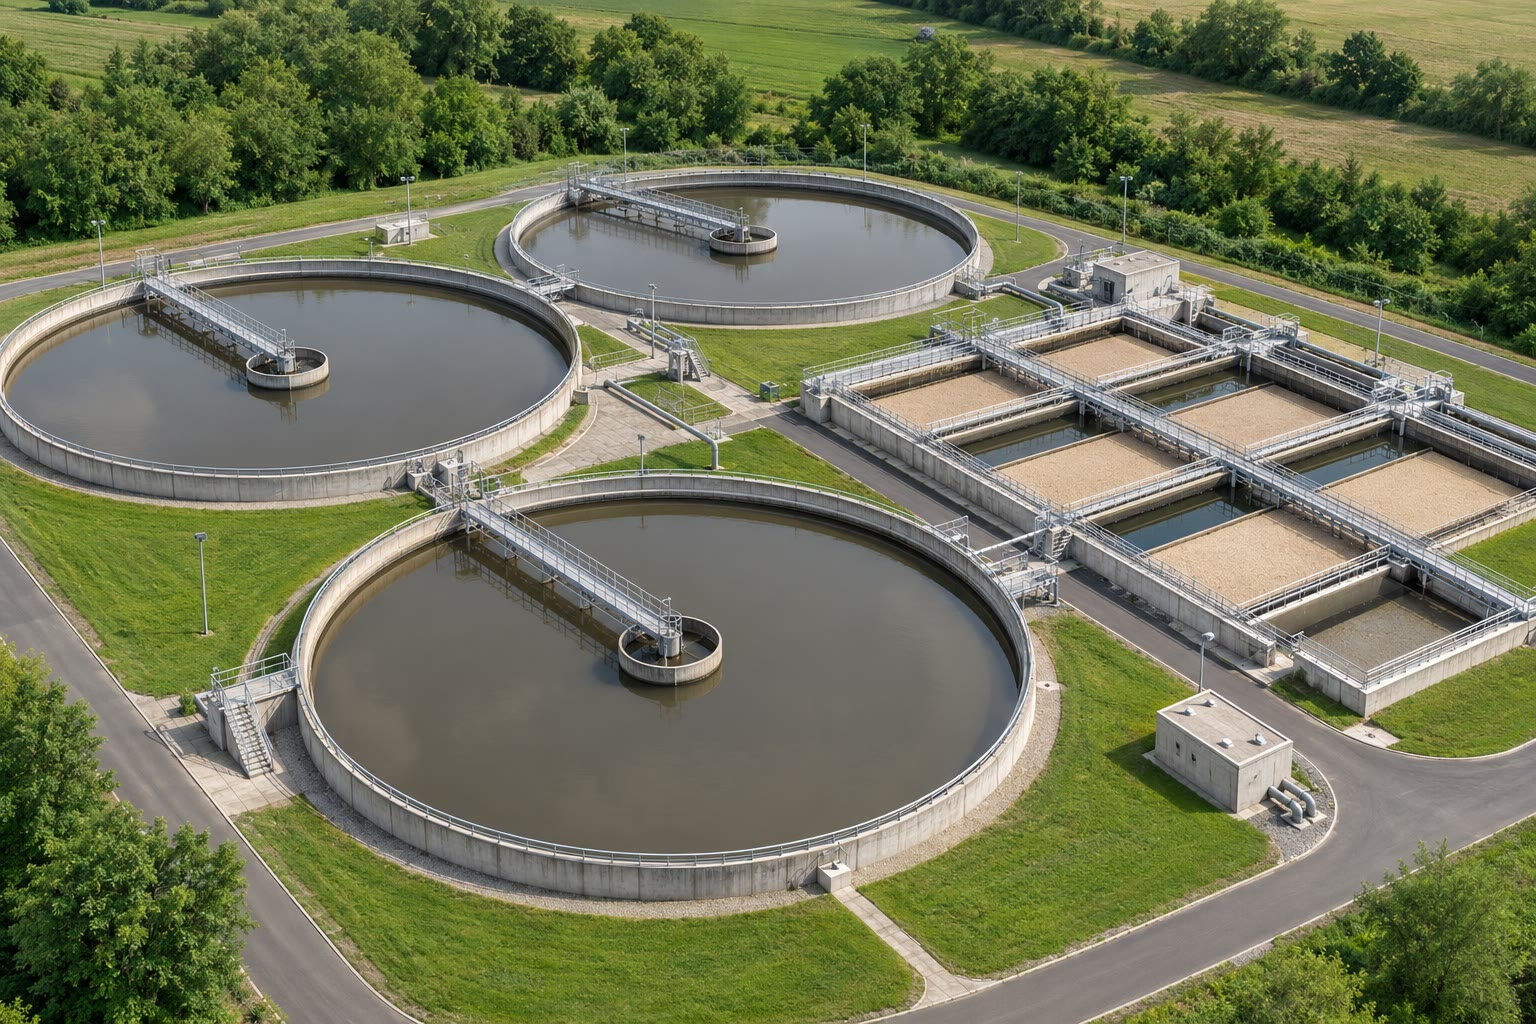
\includegraphics[width=\linewidth,height=4.6cm,keepaspectratio]{images/book1/ai/g3-settling-tanks.jpg}

{\small \omterm{def:g3:separating-mixtures:decant}{Settling} tanks of a water-treatment plant.}
\end{minipage}\hfill
\begin{minipage}[t]{0.48\linewidth}\centering
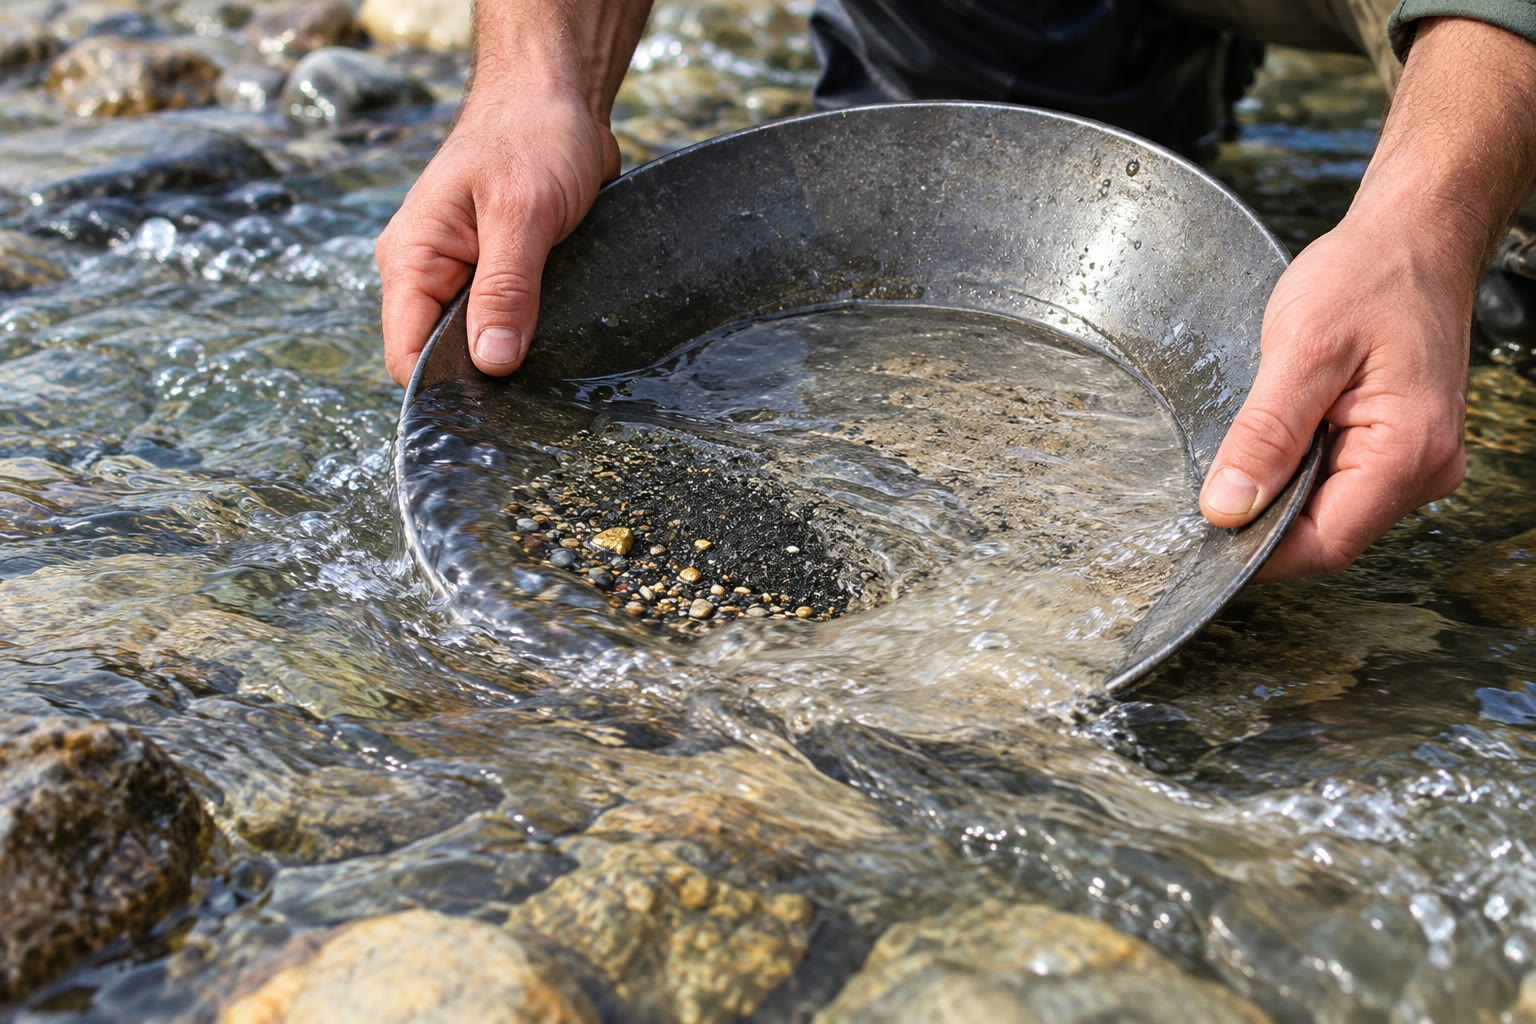
\includegraphics[width=\linewidth,height=4.6cm,keepaspectratio]{images/book1/ai/g3-gold-panning.jpg}

{\small Panning for gold: the river water carries the light sand away;
the heavy grains stay in the pan.}
\end{minipage}
\end{omfigure}

\begin{remark}[Clear is not always clean]\label{rem:g3:separating-mixtures:clean}
Water that has been filtered can look perfectly clear and still contain
dissolved substances, and germs far too small to see. That is why
nobody drinks water from a puddle or a stream, even after \omterm{def:g3:separating-mixtures:filter}{filtering} it.
\end{remark}

\section{Exercises}

\begin{exercise}[$\star$]\label{exo:g3:separating-mixtures:1}
Which method would you use to separate peas from rice grains?
\end{exercise}

\begin{exercise}[$\star$]\label{exo:g3:separating-mixtures:2}
A glass of muddy water is left on a table for an hour. What happens to
the soil? What is this called?
\end{exercise}

\begin{exercise}[$\star$]\label{exo:g3:separating-mixtures:3}
What is a \omterm{def:g3:separating-mixtures:filter}{filtrate}? Give the \omterm{def:g3:separating-mixtures:filter}{filtrate} when coffee is made.
\end{exercise}

\begin{exercise}[$\star$]\label{exo:g3:separating-mixtures:4}
Salty water is poured through a filter paper. Is the \omterm{def:g3:separating-mixtures:filter}{filtrate} salty?
Explain.
\end{exercise}

\begin{exercise}[$\star$]\label{exo:g3:separating-mixtures:5}
How can the sugar be got back from a glass of sugar water?
\end{exercise}

\begin{exercise}[$\star$]\label{exo:g3:separating-mixtures:6}
Look at the figure of the sieve. Which pieces stay in the sieve? Why do
the others fall through?
\end{exercise}

\begin{exercise}[$\star$]\label{exo:g3:separating-mixtures:7}
Match each \omterm{def:g2:mixing-and-dissolving:mix}{mix} with a method --- \omterm{def:g3:separating-mixtures:sieve}{sieving}, \omterm{def:g3:separating-mixtures:filter}{filtering} or \omterm{def:g3:separating-mixtures:evaporate}{evaporating}:
(a) sand and pebbles; (b) chalk powder in water; (c) salt in water.
\end{exercise}

\begin{exercise}[$\star$]\label{exo:g3:separating-mixtures:8}
Look at the figure of the water-treatment plant. How many steps does
the water go through? Which step removes the mud?
\end{exercise}

\begin{exercise}[$\star$]\label{exo:g3:separating-mixtures:9}
Put these steps in order to get back the sand and the salt from a jar of
sand, salt and water: evaporate the \omterm{def:g3:separating-mixtures:filter}{filtrate}; filter; collect the sand
from the paper.
\end{exercise}

\begin{exercise}[$\star\star$]\label{exo:g3:separating-mixtures:10}
Can a filter make sea water fit to drink? Explain why not.
\end{exercise}

\begin{exercise}[$\star\star$]\label{exo:g3:separating-mixtures:11}
Tea leaves are left in a teapot full of tea. Name two methods, seen in
this chapter, that separate the tea from the leaves.
\end{exercise}
